\documentclass[tikz, crop, border = {2pt 2pt 2pt 2pt}]{standalone}

\usepackage{concmath-otf}
\usetikzlibrary{decorations.pathreplacing}
\usetikzlibrary{angles, quotes, calc}

\begin{document}
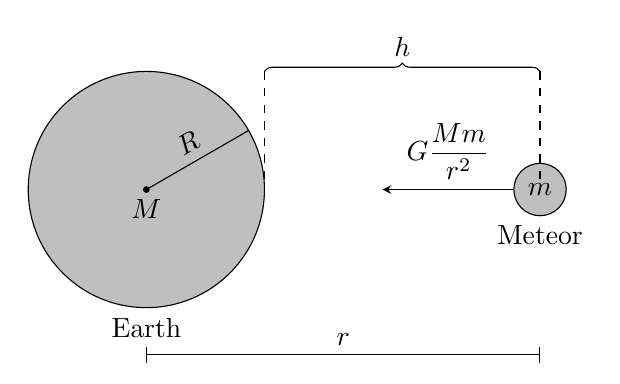
\begin{tikzpicture}
    \node[fill = lightgray, draw, inner xsep = 1.5cm, circle] (E) at (0, 0){};
    \node[below] at ($(E.south)$){Earth};
    \node[below] at (E){$M$};

    \node[fill = lightgray, draw, circle] (m) at (5, 0){$m$};
    \node[below] at ($(m.south)$){Meteor};

    \draw (0, 0) -- (30:1.5) node[midway, auto, sloped]{$R$};
    \filldraw (0, 0) circle (1pt);

    \draw[|-|] (0, -2.1) -- ++ (5, 0) node[midway, auto]{$r$};
    \draw[decorate, decoration = {brace, amplitude = 3pt}] (1.5, 1.5) -- ++ (3.5, 0) node[midway, above = 2pt]{$h$};
    \draw[dashed] (5, 1.5) -- (5, 0) (1.5, 1.5) -- (1.5, 0);

    \draw[-stealth] (m) -- ++ (-2, 0) node[midway, above]{$\displaystyle G\frac{Mm}{r^2}$};
\end{tikzpicture}
\end{document}